\chapter{Design} \label{design_chapter}
\thispagestyle{main} % Needed for Footer and Header on Chapterpage
The word design is defined as:

Do or plan (something) with a specific purpose in mind. \cite{design_definition}

This chapter therefore outlines the most important purposes the Bazo Virtual Machine and the parser are built for. It also describes the goals, requirements and restrictions of the integration of the VM into the miner and the orientation taken while building the foundation for the creation, deployment and execution of smart contracts.

\section{Virtual Machine}
When building the VM the most important design aspects

\pagebreak

\begin{figure}[H]
	\begin{center}
	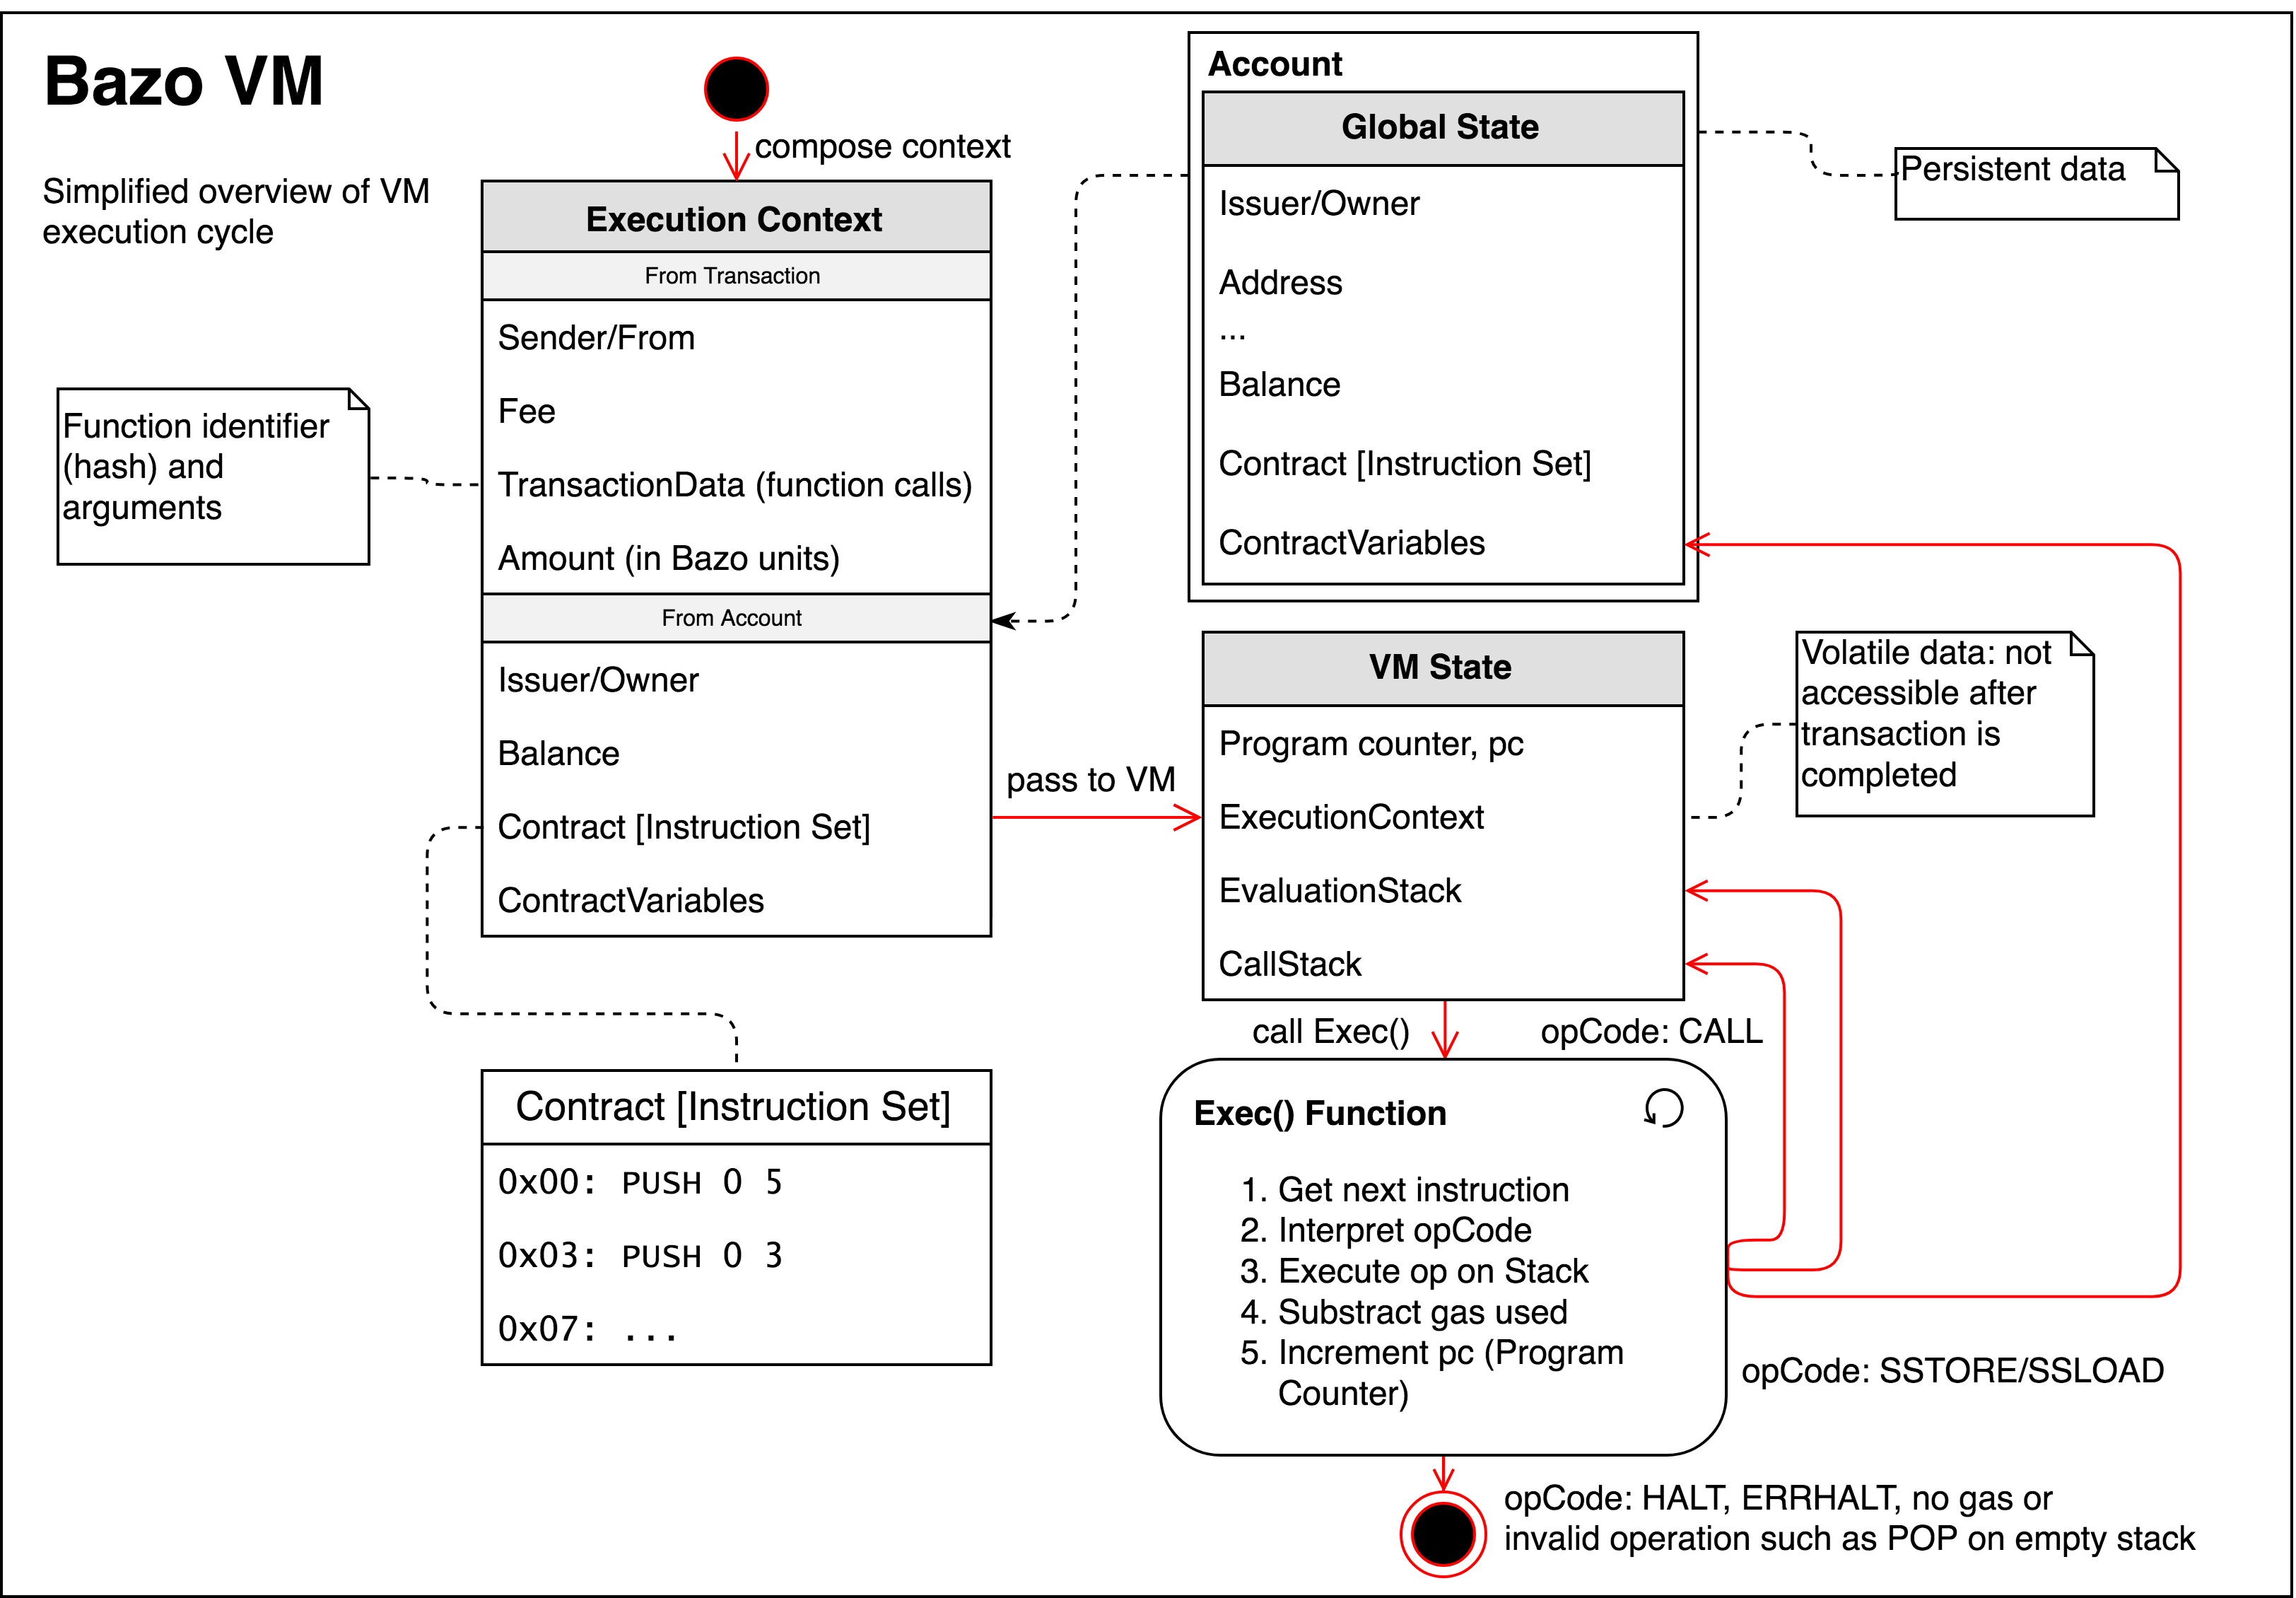
\includegraphics[width=\textwidth]{./images/execution-cycle}
	\caption{Virtual machine execution cycle}
	\label{vmexecutioncycle}
	\end{center}
\end{figure}

\subsection{Guidelines}
As the Bazo VM continues to be improved or extended by other works it was paid careful attention to make the software readable, testable, changeable and extendable. 

\begin{tabular}[t]{ p{3cm} p{12.5cm}}
\raggedright
\textbf{Readability} &
In order to make the code readable code reviews and refactorings according to the results of the review have been made. \\ \\

\raggedright
\textbf{Testability} &
Generally the code has been written using test driven development, which required writing testable code. In later stages of the project this was hugely useful and made necessary refactorings easier. \\ \\
 
\raggedright
\textbf{Extendability and Changeablity} &
The code should be structured and decoupled enough to make necessary changes or extensions to opcodes relatively easy for follow up works. As described before, having many tests makes the refactoring of the code easier. \\ \\ 
\end{tabular}

\subsection{Fault Tolerance}
As the VM just executes the instructions it receives it could easily enter an error state and panic. Already from at the begin of the work it was clear that it is critical to let the VM fail contract execution gracefully without terminating the whole miner. As a result many guards in front of functions which could panic have been placed and which return error values. The error values of the functions are then pushed on top of the VM stack if the error occurs. To test this a fuzz test has been create which executes random instructions on the VM and reports if the VM panics. 

\subsection{Maximize Human Participation in Resolving Contract Errors}
While creating the tests for the VM, especially the integration tests with the more complicated contracts, it became clear that it is necessary to include important information such as the kind of instruction that failed and what happened in the error message. As the Virtual Machine itself does not have the knowledge to resolve failures of contract execution, the error handling is pushing a error message which contains the failure and the kind of opcode that failed. How this looks is shown in Figure \ref{pushtestfailure}, which shows the error message pushed on the top of stack, when making the code of a test fail.

\begin{figure}[H]
	\begin{center}
	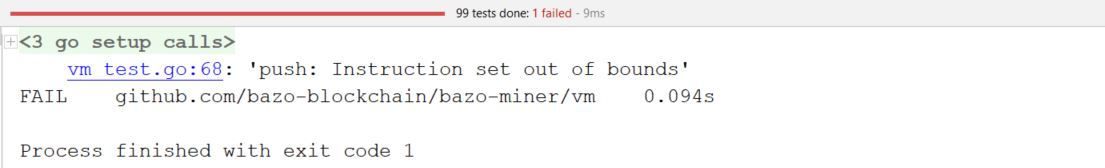
\includegraphics[width=\textwidth]{./images/push-test-failure}
	\caption{Example of an error message.}
	\label{pushtestfailure}
	\end{center}
\end{figure}

\subsection{Types of virtual machines}
There are two types of virtual machines. On the one hand there are register based virtual machines. Examples of register based virtual machines are the Lua VM and the Dalvik VM. On the other there are stack based virtual machines. The Java Virtual Machine and the .NET CLR are both stack based virtual machines. \cite{stackvsregistervm}

\begin{tabular}[t]{ p{3cm} p{12.5cm}}
\raggedright
\textbf{Register based} &
The data structure of where the operands are stored is based on registers of the CPU, therefore the instructions need to contain the addresses (registers) of the operands. This leads to longer instructions. Figure \ref{register vm} shows how adding two number works on a register based virtual machine. \cite{stackvsregistervm} The instruction is \mintinline{tasm}{ADD R1 R3 R2}.
\end{tabular}
\begin{figure}[H]
	\begin{center}
	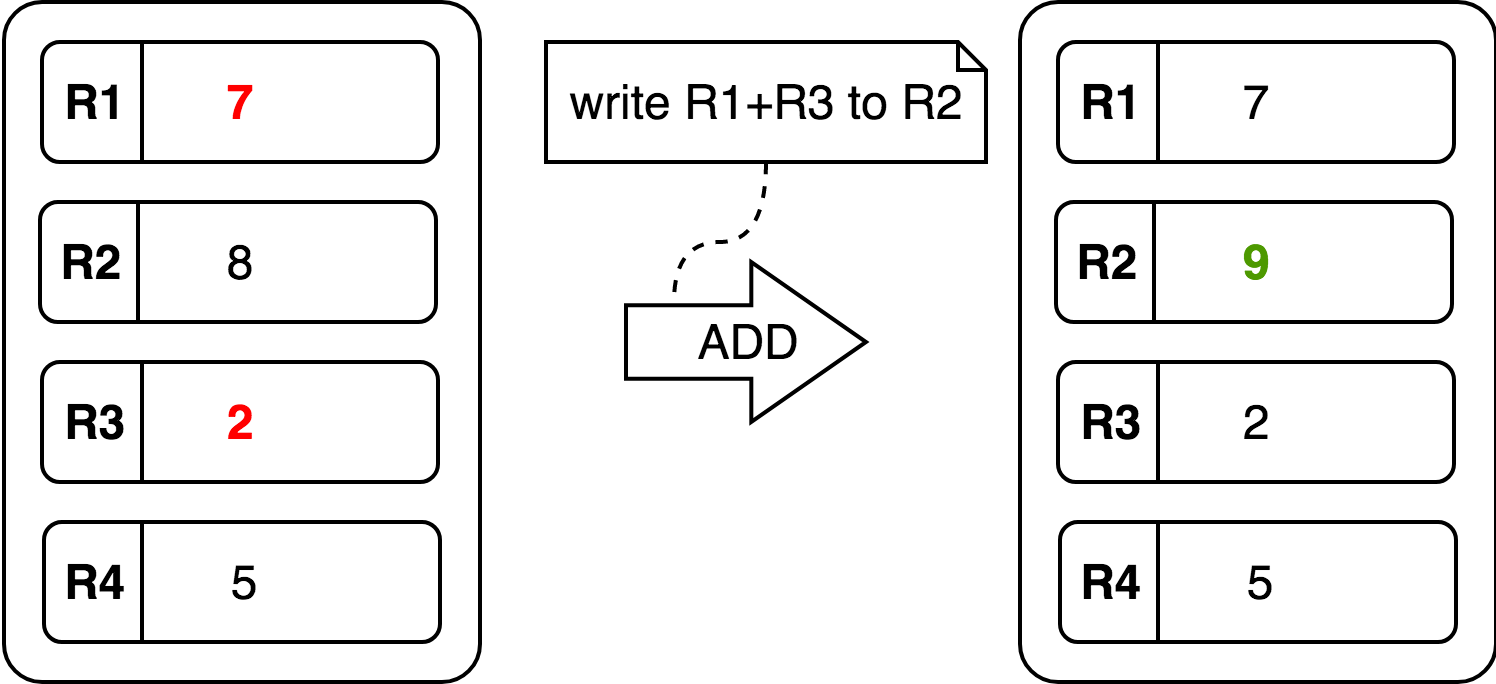
\includegraphics[width=0.61\textwidth]{./images/register-example}
	\caption{Register based virtual machine}
	\label{register vm}
	\end{center}
\end{figure}

\begin{tabular}[t]{ p{3cm} p{12.5cm}}
\raggedright
\textbf{Stack based} &
A stack based virtual machine is based on a LIFO (last in, first out) stack. Operations are carried out by popping and pushing back results on the stack. The main advantage is a stack pointer that implicitly addresses the operands, which means that no addresses are passed in instructions. The instructions code is longer since \mintinline{tasm}{POP} and \mintinline{tasm}{PUSH} instructions have to be included to retrieve and store the operands. \cite{stackvsregistervm} The instruction to add two numbers as shown in figure \ref{stack vm} are: 
\end{tabular}
\begin{figure}[thp]%
    \centering
	\begin{minipage}{0.4\textwidth}
  \begin{minted}	[
	frame=lines,
	framesep=2mm,
	baselinestretch=1.2,
	fontsize=\footnotesize,
	linenos
	]
	{tasm}
	POP
	POP
	ADD
	PUSH
  \end{minted}
  \end{minipage}
  \end{figure}
  \begin{figure}[H]
	\begin{center}
	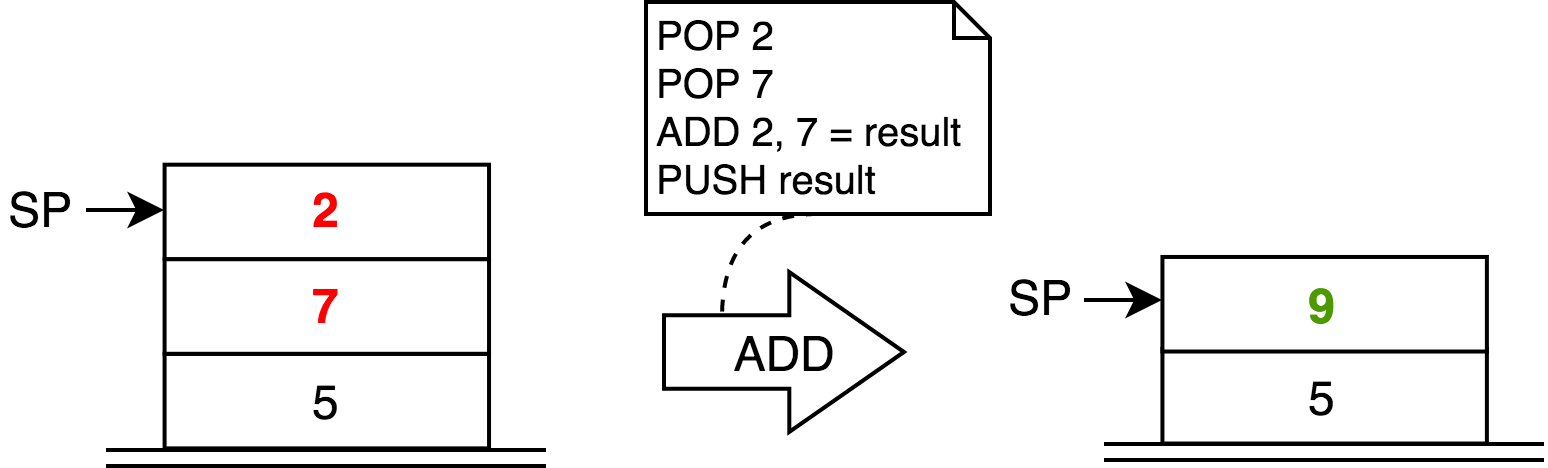
\includegraphics[width=0.6\textwidth]{./images/stack-example}
	\caption{Stack based virtual machine}
	\label{stack vm}
	\end{center}
  \end{figure}

\subsection{Design decision}
Despite the register based virtual machine having advantages such as more possibilities for optimizations and having no overhead from pushing and popping, over a stack based virtual machine we decided to implement a stack based virtual machine. This decision was most influenced by the implementation of related projects, namely Ethereum and NEO. Besides that, the implementation of a stack based virtual machine is simpler and much more resources are available.

\section{Contract deployment}

\begin{tabular}[t]{ p{3cm} p{12.5cm}}
\raggedright
\textbf{State of the Art} &
Other blockchains such as Ethereum allow to create and deploy a contract over an IDE. These contracts can be written in a high level language and they can be deployed automatically. In this work the foundation for smart contract deployment and execution has been laid out and designed accordingly. To make it as easy for the end user as mentioned above, a lot more work and resources would have to be invested. \\ \\

\raggedright
\textbf{Current Contract Deployment} &
Currently contracts are account transactions and as Bazo is permissioned, have to be created with the root key pair. These transactions are added to the unprocessed account transactions pool in the storage of the miner directly. When creating the account transaction, the contract and the initial values of the contract have to be provided. The miner then validates the transaction and creates a contract account. The integration tests of the deployment and execution of smart contracts have been setup in this manner.  \\ \\

\raggedright
\textbf{Restrictions} &
This means that yet only developers can create new contracts. \\ \\

\raggedright
\textbf{Rationale} &
To make contract creation available for account owners, it would have to be possible to create a contract account with any valid key pair of a Bazo account. Also the peer 2 peer package would have to support the features implemented during this work.
Both tasks by themselves would have exceeded the scope of this thesis. \\ \\
\end{tabular}

\section{Execution of a contract method}
\begin{tabular}[t]{ p{3cm} p{12.5cm}}
\raggedright
\textbf{State of the Art} &
In other blockchains such as Ethereum, smart contracts can be called via the wallet or the web api. The results can be checked via api, wallet or block explorer. \\ \\
\raggedright
\textbf{Current Contract Execution} &
In Bazo a transaction which calls a contract has to be added to the unprocessed transactions pool. The miner takes the transaction out of the pool and validates it. As the data field of the transaction is set, it will setup the vm context and execute the called function in the vm. After a successful execution, the changed contract variables are written back \\ \\

\raggedright
\textbf{Restrictions} &
As the features are not yet implemented in the client it is not possible to send this kind of transaction via the web api of the miner. It is also not yet possible to check the result, since smart contracts are not part of the block explorer. \\ \\

\raggedright
\textbf{Rationale} &
Implementing the features in the other applications as well would have exceeded the scope of this work. \\ \\
\end{tabular}

\pagebreak

\section{VM Integration} \label{design_miner}
As mentioned before, the miner is responsible for processing and validating transactions. This section describes the requirements and restrictions the integration of the virtual machine is based on. Furthermore, the changes that were made to the miner are documented.

\subsection{Transaction Types} \label{transactionTypes}
The miner comes with different transaction types.

\begin{tabular}[t]{ p{3cm} p{12.5cm}}
\raggedright
\textbf{FundsTx} &
This type of transaction is used to transfer Bazo coins from one account to another and can be used by any externally owned account.\cite{ba_miner} For this reason it was extended with a Data field to enable users to call smart contract functions.
\\ \\
\end{tabular}

\begin{figure}[thp]%
    	\centering
		\begin{minipage}{0.4\textwidth}
		\begin{minted}
		[
		frame=lines,
		autogobble,
		framesep=2mm,
		baselinestretch=1.2,
		fontsize=\footnotesize,
		linenos
		]
		{go}
		type FundsTx struct {
			Header byte
			Amount uint64
			Fee    uint64
			TxCnt  uint32
			From   [32]byte
			To     [32]byte
			Sig1   [64]byte
			Sig2   [64]byte
			Data   []byte
		}
		\end{minted}
		\end{minipage}
\end{figure}

\begin{tabular}[t]{ p{3cm} p{12.5cm}}
\raggedright
\textbf{AccTx} &
The account transaction is used to create a new account. As for now this type of transaction is only allowed to root accounts, since the signature has to be signed with the private key of a root account. \cite{ba_miner} Nevertheless this transaction type is the perfect foundation to create smart contract accounts. Therefore a contract field and a contract variable field were added. \\ \\
\end{tabular}

\begin{figure}[thp]%
    	\centering
		\begin{minipage}{0.4\textwidth}
		\begin{minted}
		[
		frame=lines,
		autogobble,
		framesep=2mm,
		baselinestretch=1.2,
		fontsize=\footnotesize,
		linenos
		]
		{go}
		type AccTx struct {
			Header            byte
			Issuer            [32]byte
			Fee               uint64
			PubKey            [64]byte
			Sig               [64]byte
			Contract          []byte
			ContractVariables []big.Int
		}
		\end{minted}
		\end{minipage}
\end{figure}

\begin{tabular}[t]{ p{3cm} p{12.5cm}}
\raggedright
\textbf{ConfigTx} &
This type of transaction is used to change system parameters such as block size, block interval or minimum fee.  For more information about this transaction type, see the thesis of Livio Sgier \cite{ba_miner}. \\ \\
\textbf{StakeTx} &
Since the Bazo Blockchain is in transition from proof of work to proof of stake consensus mechanism there is a StakeTx transaction type. This type of transaction is continuously being improved. For more information refer to the theses of Simon Bachmann \cite{ba_pos} and Marc-Alain Chételat \cite{ba_client}.
\end{tabular}

\subsection{Accounts} \label{accounts}
An account is the result of processing an account transaction. Accounts are objects on the heap of the miner. Figure \ref{struct_account} shows the struct for Account.

\begin{figure}[thp]%
    	\centering
		\begin{minipage}{0.6\textwidth}
		\begin{minted}
		[
		frame=lines,
		autogobble,
		framesep=2mm,		baselinestretch=1.2,
		fontsize=\footnotesize,
		linenos
		]
		{go}
		type ByteArray []byte

		type Account struct {
			Address            [64]byte  // 64 Byte
			Issuer             [32]byte  // 32 Byte
			Balance            uint64    // 8 Byte
			TxCnt              uint32    // 4 Byte
			IsStaking          bool      // 1 Byte
			HashedSeed         [32]byte  // 32 Byte
			StakingBlockHeight uint32    // 4 Byte
			Contract           []byte
			ContractVariables  []ByteArray
		}
		\end{minted}
		\caption{Stack based virtual machine}
		\label{struct_account}
		\end{minipage}
\end{figure}

\begin{tabular}[t]{ p{3cm} p{12.5cm}}
\raggedright
\textbf{Externally Owned Accounts} &
Externally owned accounts are accounts that are owned by the person who has access to the combination of the public and private key. Having both, the person is able to execute transaction from that account. The creation of externally owned accounts was already given by the previous thesis written by Livio Sgier. An externally owned account does not have an Issuer, Contract and ContractVariables. \\ \\
\textbf{Smart Contract Accounts} &
Smart contracts accounts are created and owned by externally owned accounts. Smart contracts accounts have two additional fields, which were added to the account creation transaction. The Issuer shows which externally owned account issued the contract account. A contract account has both, Contract and ContractVariables, fields set.

	\begin{description}
  		\item[Contract] This field contains the smart contract in byte code. The data type is byte slice, since contracts have variable lengths.
  		\item[ContractVariables] This field contains the state variables that can be altered by contract functions. The data type is a slice of byte slices, since a contract can have a multiple variables.
	\end{description}
\end{tabular}

\subsection{Consistecy}
Since the blockchain is a distributed database and the VM is allowed to change the data of the database eventually, consistency was a very important aspect of the design of its integration. In order to keep the data of the miner consistent even after potential failure of the VM, the context in which the VM is exectued is created by the miner and passed to the VM. Especially important hereby is letting the vm only work on copies and letting the VM only work on immutable values in order to avoid an encapsulation breach where the VM adjusts a reference value used by the actual miner. If the VM executes without an error the miner writes the changes back by itself. Therefore in the case of an error the copies just have to be discarded, which is a lot easier than resetting the changed variables back to the old values

\section{Parser}
Since writing all contracts directly in byte code can be very complicated and time-consuming, we decided to write a very basic parser. The goal of the parser was to make writing contracts easier by allowing the usage of labels and comments. Having labels resolves the problem of counting addresses when using flow operation opcodes like \mintinline{yaml}{JMP} and \mintinline{yaml}{CALL} since they generally take an address as argument and change the program counter accordingly. Labels could also be interpreted as jump markers. The parser could also be used as foundation for building a compiler which translates a contract written in a high-level language into Bazo byte code. For the rest of this thesis the code that can be interpreted by the parser is referred to as \flqq Enhanced Bazo Byte Code\frqq{} and the code the virtual machine operates on and which is stored on the blockchain as \flqq Bazo Byte Code\frqq.

\subsection{\flqq Enhanced Bazo Byte Code\frqq{}}
Listing \ref{basiccontract_design} shows an example of a contract written in \flqq Enhanced Bazo Byte Code\frqq{}. It is possible to have single line comments and inline comments as well, as seen in line 1 and line 5. Comments and empty lines are ignored by the parser. The first word in line is either an opcodes or a label, which ends with a colon. Opcodes are optionally followed by arguments. It is predefined what type of arguments an opcode has. The \mintinline{go}{CALL} opcode in line 4 for instance takes a label and a byte as argument.

\begin{figure}[thp]%
    \centering
	\begin{minipage}{0.6\textwidth}
\begin{minted}
[
	frame=lines,
	framesep=2mm,
	baselinestretch=1.2,
	fontsize=\footnotesize,
	linenos
]
{yaml}
# This is a simple program which calls a function
PUSH 55780
PUSH 5
CALL addNums 2
HALT # stops execution

addNums:
LOAD 0
LOAD 1
ADD
RET
\end{minted}
\end{minipage}
\caption{Basic contract with function call written in \flqq Enhanced Bazo Byte Code\frqq{}}
\label{basiccontract_design}
\end{figure}

\subsection{Compile process}
First the parser splits the contract written in \flqq Enhanced Bazo Byte Code\frqq{}, which is basically only a long string, into tokens. A token consists of a token type and a value. The token type represents a kind of lexical unit e.g. opcode, label or a sequence of input characters. The token types are the symbols that are processed by the parser. \cite{aho_compilers:_2007} To get to the \flqq Bazo Byte Code\frqq{} the resulting set is iterated and the token is replaced by the corresponding byte value.

\section{Smart contracts}
Smart contracts are programs that are stored on the blockchain. A smart contract consists of an ABI (application binary interface) and one or more callable functions. Smart contracts are deployed through a transaction (AccTx). Calling a certain function is also made through a transaction (FundsTx). When someone wants to call a certain function in a smart contract, a special transaction to the public address of the smart contract is executed. The transaction contains an identifier in a designated data field, so the ABI can match the identifier with the function the caller wants to execute. Arguments passed to that function are also transmitted in that field. Since a transaction is processed simultaneously on all nodes of the network, all functions have to be deterministic.

\subsection{Coding smart contracts}
Smart contracts for the NEO blockchain can be coded in C\#, Java, Kotlin, F\# or Python. There are different ways to create an Ethereum smart contract. There are different high-level programming languages that can be compiled to Ethereum byte code. Solidity is being developed by the Ethereum community and is the industry standard. Solidity is heavily inspired by JavaScript with the idea to attract JavaScript developers to write smart contracts. In this section a simple contract is written once in Solidity and once in Bazo byte code instructions.

\subsubsection{Sample smart contact in Solidity}
%\begin{lstlisting}[caption={Solidity contract},captionpos=b,label={lst:dialogex}]

%\end{lstlisting}
\begin{figure}[thp]%
    \centering
	\begin{minipage}{0.5\textwidth}
\begin{minted}
[
	frame=lines,
	framesep=2mm,
	baselinestretch=1.2,
	fontsize=\footnotesize,
	linenos
]
{javascript}
contract MyFirstContract {
  uint myData; //State variable

  function set(uint x) public {
    myData = x;
  }

  function add(uint amount) public {
    myData += amount;
  }

  function sub(uint amount) public {
    myData -= amount;
  }

  function get() public constant returns (uint) {
    return myData;
  }
}
\end{minted}
\end{minipage}
\end{figure}

This contract has the state variable myData. Calling the function set() with an uint parameter sets the variable. Calling the function add or sub allows the transaction sender to either add or subtract a certain amount from that variable. In order to call a function a transaction must be executed.
\pagebreak

\subsubsection{Sample smart contract in Bazo-vm byte code instructions}
Compiled Smart Contract with ABI would look like this:
\begin{figure}[thp]%
    \centering
	\begin{minipage}{0.7\textwidth}
\begin{minted}
[
	frame=lines,
	framesep=2mm,
	baselinestretch=1.2,
	fontsize=\footnotesize,
	linenos
]
{yaml}
CALLDATA        # Puts the arguments passed to the smart contract
                # and the function hash on top of stack
# ABI:
DUP
PUSH set
EQ
JMPIF set

DUP
PUSH add
EQ
JMPIF add

DUP
PUSH sub
EQ
JMPIF sub

HALT

:set            # set function
SSTORE myData   # stores the variable in ContractVariables
HALT

:add            # add function
POP
SLOAD myData    # loads the variable and puts a local copy on the stack
ADD
SSTORE myData   # overwrites the variable in ContractVariables
HALT

:sub            # sub function
...
\end{minted}
\end{minipage}
\end{figure}

\section{Execution context}
With data coming from the transaction, the account and the miner the Execution Context is composed. The Execution Context contains all the data needed to start the execution cycle. Every field is needed and/or can be used by the virtual machine. We use the pattern parameterize from above and encapsulate copies of all the variables we want to access in a context object.

Providing specific byte code instructions that put the value of a certain field on the top of the stack smart contract, functions that for instance can only be called by the owner of the smart contract account or functions that only can be executed if the balance is enough can be created.

\subsection{Data from transaction}
\begin{description}
  \item[Sender/Address] The sender field shows the transactions sender public address.
  \item[Fee] The maximum price the transaction can cost.
  \item[TransactionData] This field contains the identifier to the function the sender wants to call on a certain smart contract and its arguments. In order to identify the function and still being able to override functions and enable polymorphism, the identifier is a hash build from the function signature (name and parameters).
  \item[Amount] This field shows the amount of Bazo units send in this transaction.
\end{description}

\subsection{Data from receiver account}
\begin{description}
  \item[Issuer/Owner] This field contains the public address of the account owner.
  \item[Balance] This field contains the amount of coins this account owns.
  \item[Contract] This field is the smart contract itself and contains the byte code. The datatype is \mintinline{yaml}{[]byte}, so it can easily be packed into a transaction field.
  \item[ContractVariables] This field contains the state variables that are changed by executing transactions.
\end{description}

\subsection{Data from miner}
\begin{description}
  \item[Block header] This field is needed for block number/hash
\end{description}

\section{Fee} \label{fee}
Running a node in the network carries costs and the node operators want to be compensated. The fee is expressed in the smallest unit of Bazo coins available. The cost of execution vary since depending on the complexity of the function the amount of time which the whole network is busy processing differs. Ethereum calculates the cost depending on which instructions (such as \mintinline{yaml}{ADD} known from assembler) are used. In Ethereum and Neo this fee is called gas. Bitcoin calculates the cost depending on the size of the transaction. We combine both concepts with the goal of simplifying the calculation of the execution fee.

The fee is also a way to secure the network. As mentioned before the execution must be deterministic. Using a JUMP instruction (changing the program counter of the execution) a smart contract creator could develop a smart contract function containing an endless-loop, which then he could call, causing the network to jam and not accepting new transactions because the execution doesn't come to an end. With the introduction of gas subtracted with every instruction once no more gas is available the processing of the transaction is aborted.
